\section{Wavelets}
\subsection{Allgemein \baeni{19}}
  Wavelet-Funktionen werden auch als \em Mother-Funktionen \em bezeichnet.
  \[
    \psi(t) = \psi_{0,0}(t)
  \]
 
  Davon werden gestreckte ($m>0$)/gestauchte ($m<0$) und verschobene (rechts: $n > 0$, links: $n < 0$) Funktionen hergeleitet:
  \[  
    \psi_{m,n}(t)=\frac{1}{\sqrt{2^m}} \cdot \psi\left(\frac{t}{2^m} - n\right) = 2^{-m/2} \cdot \psi(2^{-m}t-n) \quad m,n \in \mathbb{Z}
  \]
  Diese erfüllen die L2-Norm 1: $|| \psi_{m,n} ||^2 = \int_{-\infty}^{\infty} |\psi_{m,n}(t)|^2 dt = 1$ und sind orthonormiert: $<\psi_{m,n}, \psi_{m',n'}> = 0$, wenn $m \neq m'$ oder $n \neq n'$. Deren Mittelwert ist 0 (das 0. Moment ist verschwindend): $\int_{-\infty}^{\infty} \psi_{m,n}(t) dt = 0$.

\subsection{Haar Wavelets \baeni{19}}
\begin{center}
	\begin{minipage}[c]{0.65\textwidth}
    \begin{center}
    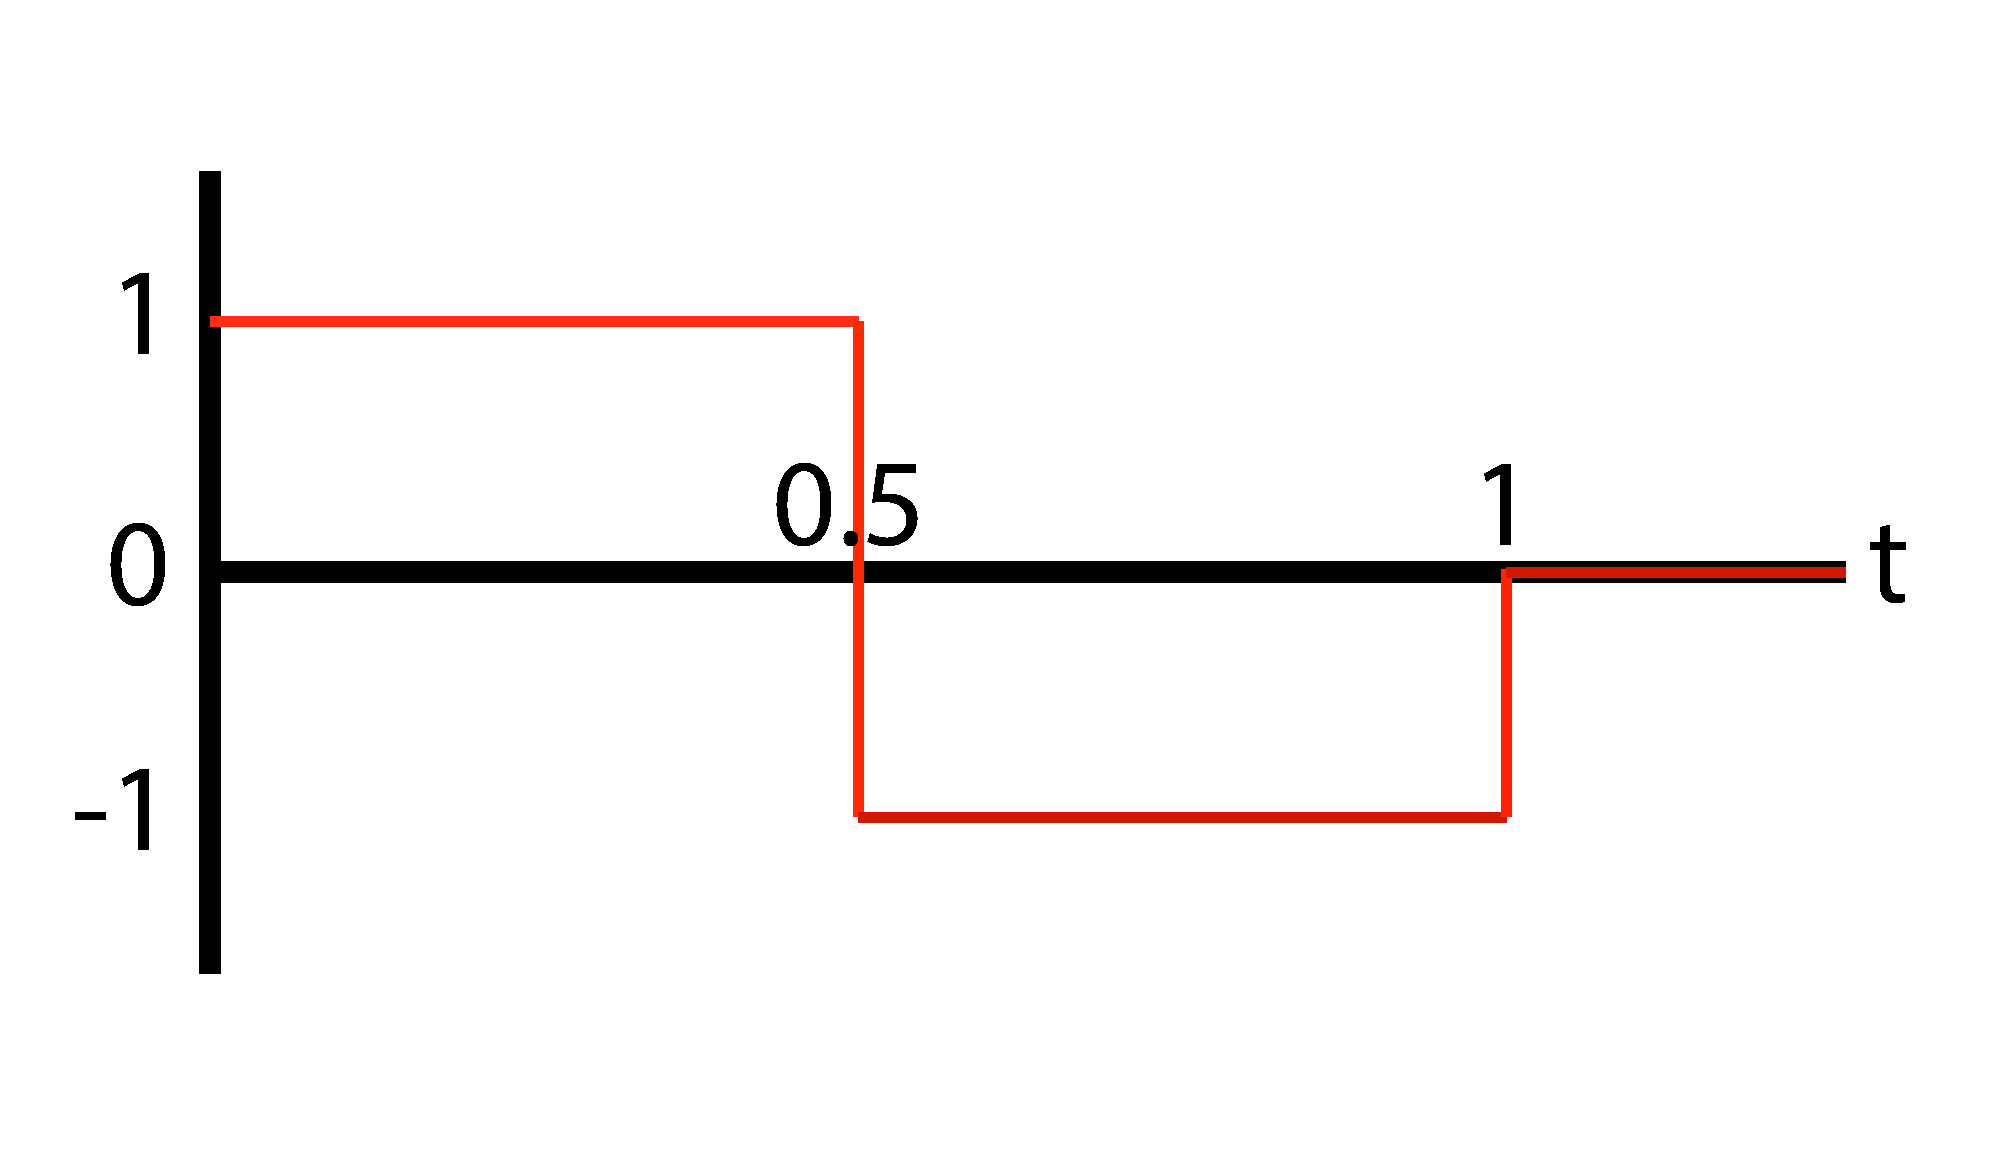
\includegraphics[width=6cm]{content/HaarWavelet.pdf}
    \end{center}
    \[
      \psi(t) = \psi_{0,0}(t)=\begin{cases} 1 \quad 0 \leq t < \frac{1}{2}\\ -1 \quad \frac{1}{2} \leq t < 1  \end{cases}
    \]
    
    \[	\psi_{m,n}  = \begin{cases} 
    	\frac{1}{\sqrt{2^m}} \qquad 2^m n \leq t < 2^m(n+\frac{1}{2}) \\ 
    	\frac{-1}{\sqrt{2^m}} \qquad 2^m(n+\frac{1}{2}) \leq t < 2^m(n+1)
    	\end{cases}
    \]
    
	\end{minipage}
	\begin{minipage}{0.3\textwidth}
	\textbf{Haar-Wavelets gestreckt, gestaucht und geschoben}\\
	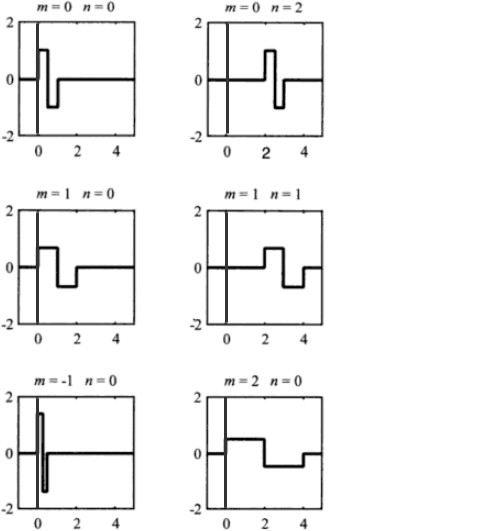
\includegraphics[width=7cm]{./content/HaarStretchedMoved}
	\end{minipage}
\end{center}



\[ 
	\nu_{m,n} = \langle \psi_{m,n} | f \rangle = \int\limits_{-\infty}^{\infty}\psi_{m,n}(t) \cdot f(t) \,\mathrm{d}t = 
	\dfrac{1}{\sqrt{2^m}} \left( \int\limits_{2^mn}^{2^m(\frac12+n)} f(t) \mathrm{d}t - \int\limits_{2^m(\frac12+n)}^{2^m(1+n)}f(t) \mathrm{d}t  \right)
	\quad \Leftrightarrow \quad
	f(t)=\sum_{m,n \in \mathbb{Z}} \nu_{m,n} \cdot \psi_{m,n}
\]
\[
	||f||^2 = \sum_{m,n \in \mathbb{Z}} |\nu_{m,n}|^2 \qquad \qquad ||f-f_N||^2 = ||f - \sum_{m,n \in \mathbb{Z}}^N \nu_{m,n} \cdot \psi_{m,n}||^2 = \sum_{k=N+1}^{\infty} |c_k|^2
\]


\textbf{TI-89 Haar-Berechnungen}
\begin{alltt}
1/(\(\sqrt{}\)(2^m))*(\(\int\)(f(x),x,2^m*n,2^m*(1/2+n))-\(\int\)(f(x),x,2^m*(1/2+n),2^m*(1+n)))\(\rightarrow\)haar(m,n)
when(0\(\leq\)x,0,when(x<\(\pi\)/2,sin(x),0))\(\rightarrow\)f(x) \(\quad\) when(0\(\leq\)x,0,when(x<1,1,0))\(\rightarrow\)f(x)
haar(m,n)
\end{alltt}

\textbf{Haar-Transformation} (direkt, U5-2): 
\begin{enumerate}
	\item Funktion abtasten bei $2^m(n+1/2)$ im Intervall $[a,b] \qquad u_{m,n} = \int_{n 2^m}^{(n+1)2^m} 2^{m/2} f(t) dt \approx \sqrt{2^m}f(2^m[n+1/2])$ 
	\item Die abgetastete Sequenz mit 0 auffüllen bis zu einer Zweierpotenz
	\item In jedem Schritt $u_{m+k+1}, \nu_{m+k+1}$ berechnen
\end{enumerate}

\begin{tabularx}{\textwidth}{p{9cm}|X}
Schnelle Haar-Transformation (iterativ, \baeni{26})
  & Schnelle Haar-Rücktransformation (iterativ, \baeni{28})\\
$u_{m+1,n} = \dfrac{u_{m,2n}+u_{m,2n+1}}{\sqrt{2}}$
  & $u_{m-1,2n} = \dfrac{u_{m,n}+\nu_{m,n}}{\sqrt{2}}$ \\
$\nu_{m+1,n} = \dfrac{u_{m,2n}-u_{m,2n+1}}{\sqrt{2}}$
  & $u_{m-1,2n+1} = \dfrac{u_{m,n}-\nu_{m,n}}{\sqrt{2}}$
\end{tabularx}

\newpage
\textbf{Haarsche Filter \baeni{29}}\\
  \begin{tabularx}{\textwidth}{l |l |X}
    Bezeichnung:
      & Moving Average
      & Moving Difference \\
    Analyse-Filter
      & $A(x)_n = \frac{x_n + x_{n+1}}{\sqrt{2}} \quad
         A(z) = \frac{1+z}{\sqrt{2}}$
      & $D(x)_n = \frac{x_n - x_{n+1}}{\sqrt{2}} \quad
         D(z) = \frac{1-z}{\sqrt{2}}$ \\
    Analyse-Koeffizienten
      & $a_0 = a_{-1} = \frac{1}{\sqrt{2}}$
      & $d_0 = \frac{1}{\sqrt{2}}, d_{-1} = -\frac{1}{\sqrt{2}}$ \\
    Synthese-Filter
      & $\tilde{A}(x)_n = \frac{x_n + x_{n-1}}{\sqrt{2}} \quad
         \tilde{A}(z) = \frac{1+z^{-1}}{\sqrt{2}}$
      & $\tilde{D}(x)_n = \frac{x_n - x_{n-1}}{\sqrt{2}}
         \tilde{D}(z) = \frac{1-z^{-1}}{\sqrt{2}}$ \\
    Synthese-Koeffizienten
      & $\tilde{a}_0 = \tilde{a}_{1} = \frac{1}{\sqrt{2}}$
      & $\tilde{d}_0 = \frac{1}{\sqrt{2}}, \tilde{d}_{1} = -\frac{1}{\sqrt{2}}$ \\
    
  \end{tabularx}